\chapter{亚线性复杂度的PIR}

我们首先提出一种在半诚实环境下的两服务器PIR方案的构造。我们的构造基于CK20\cite{EC:CorKog20}框架,采用了一种新颖的方法来构建Hint和Query。该方法能够高效地进行查询,同时不会妨碍数据可靠性的集成。

\section{亚线性复杂度PIR的基本构造}
我们基于现有的亚线性PIR方案\cite{EC:CorKog20, C:LazPap23}构建可验证PIR,对这些方案的认识有助于理解本文提出的新方案。我们从如图\ref{fig:CK20}所示的两服务器PIR方案起步,讨论如何修正该协议的局限性。该协议是一个离线-在线PIR方案,我们使用$\hintserver$ 与 $\queryserver$ 两个记号来区分协议中涉及到的两台服务器。这些记号是根据两台服务器的功能定义的:

\subsection{构造方案}

\noindent \textbf{离线阶段:}
\begin{itemize}
\item \textbf{Setup:} 客户端$\client$ 生成$\hintcount$ 组集合$\setkey_j, j\in[\hintcount]$。每个集合包含$\setsize$个在范围[$\dbsize$]内的随机索引。
\item \textbf{Hint:}$\client$将这些集合转发给$Hint$服务器$\hintserver$。$\hintserver$计算这些集合对应数据库中记录的和,表示为$\hint_j \coloneqq \sum_{k\in \setkey_j} \db_k, j \in [\hintcount]$。$\client$存储这些集合及其对应的记录之和作为校验值。
\end{itemize}

\noindent \textbf{在线阶段:}
\begin{itemize}
\item \textbf{Query:}$\client$首先找出一个包含目标索引$\dbidx$的集合$\setkey_\hintidx$,并从该集合中去掉$\dbidx$,$\queryquery \coloneqq \setkey_\hintidx \setminus \{\dbidx\}$。此外,$\client$生成一个包含索引$\dbidx$的新集合$\setkey'$,并令$\hintquery \coloneqq \setkey' \setminus \{\dbidx\}$。$\client$将集合$\hintquery$发送给$Hint$服务器$\hintserver$,将$\queryquery$发送给$Query$服务器$\queryserver$。
\item \textbf{Answer:} 收到这些集合后,服务器分别为两个集合计算校验值,$\queryanswer\coloneqq \sum_{j\in \queryquery}\db_j$,$\hintanswer\coloneqq \sum_{j\in \hintquery}\db_j$,将这些校验值发送给$\client$。
\item \textbf{Reconstruct:}$\client$ 计算出所需的记录:$\db_\dbidx \coloneqq \hint_\hintidx - \queryanswer$。
\item \textbf{Refresh:}$\client$ 更新$Hint$: $\setkey_\hintidx \coloneqq \setkey'$,$\hint_\hintidx \coloneqq \hintanswer+\db_\dbidx$。
\end{itemize}


\subsection{基本构造的缺陷}
不妨先假设客户端生成的集合足够多,在$Query$阶段总能找到包含目标索引的集合。在此前提下,客户端总能得到想要查询的记录$\db_\dbidx$,该协议的正确性显而易见。然而,该协议存在三个关键问题:

\begin{enumerate}
\item \textbf{低效的集合隶属测试:} 搜索包含查询索引$\dbidx$的集合$\setkey_t$的过程计算量很大。客户端需要遍历所有集合,同时遍历集合中的元素已确定某个索引是否隶属于这个集合。尽管可以通过排序和二分查找进行优化,但它仍然需要$O(\sqrt{\dbsize}\log \dbsize)$的在线计算复杂度。
\item \textbf{低下的空间和通信效率:} 对客户端来说,以明文形式生成、存储和发送这些集合的效率低下,客户端完成协议时需要$O(\dbsize)$的存储和离线通信复杂度。粗略估计,为了确保正确性,客户端需要大约$\hintcount = O(\lambda\sqrt{\dbsize})$个集合,每个集合的大小为$\setsize = \sqrt{\dbsize}$。相应的存储和离线通信复杂度为$O(\lambda\dbsize)$。
\item \textbf{有缺陷的隐私性:} 集合$\queryquery$和$\hintquery$不可能包含查询的索引$\dbidx$。从信息论角度来看,这泄露了大约$1/(\sqrt{\dbsize}\ln 2)$比特$\dbidx$的信息。
\end{enumerate}

\subsection{虚设查询及其引入的新问题}
在现有工作中,研究者已经提出了多种方法来解决上述问题。例如,TreePIR \cite{C:LazPap23} 利用了一种称为弱可穿孔伪随机函数(Weakly Puncturable Pseudorandom Function)的原语,并引入了一种新的亚线性PIR构造。 Piano \cite{Piano} 提出了一个类似的算法,称为$PossibleParities$。然而,当尝试向这些协议中引入可验证性时,这些方案遇到了类似的困境,本文总结为“虚设查询”。

\begin{figure}
    \centering
    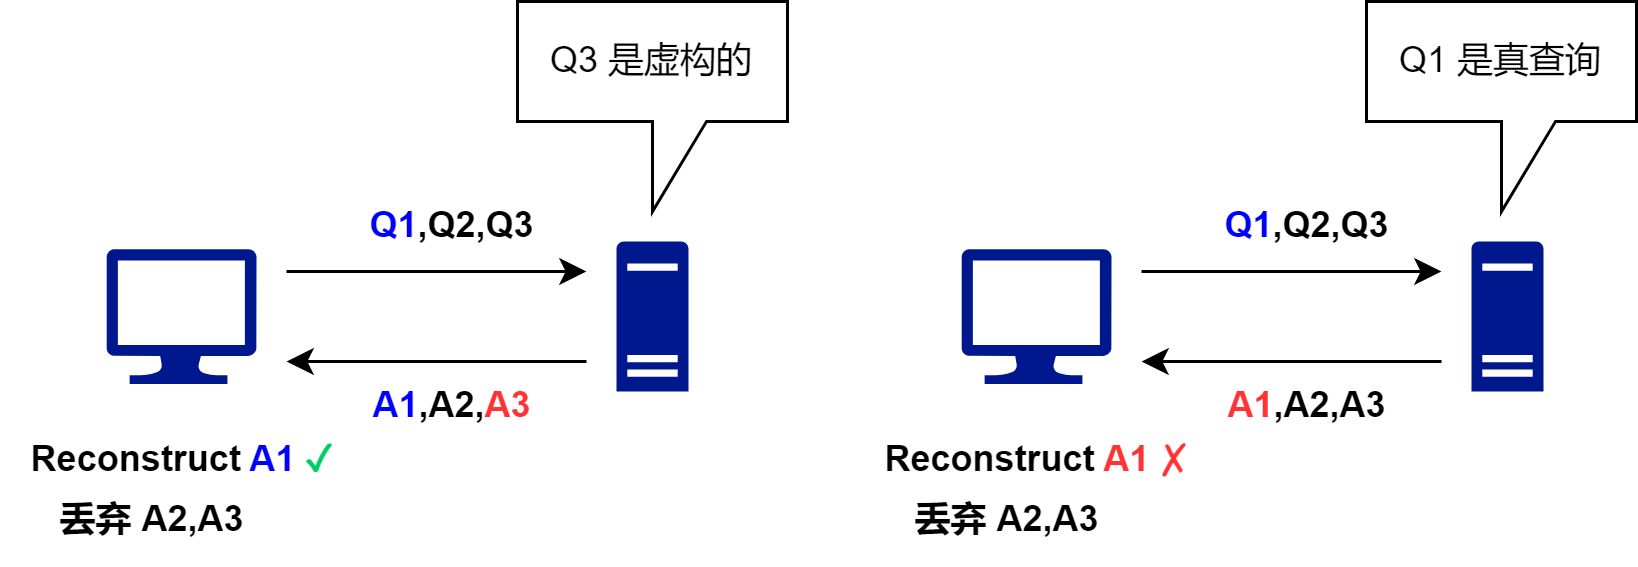
\includegraphics[width=1\linewidth]{figure/dummy.png}
    \caption{关于虚设查询的图示}
    \label{fig:dummy}
\end{figure}

这些虚设查询是随机生成的假查询,其目的是与真实查询相混淆。在这些方案中,客户端发送的单个查询会泄露关于查询索引$\dbidx$的信息给服务器。通过真实查询与虚设查询的组合,协议才得以隐藏索引$\dbidx$。服务器无法区分虚设查询与真实查询,所以会对虚设查询同样作出回应,但客户端会忽略对虚设查询的回应。

在半诚实环境下,这些方案的隐私性依赖于服务器无法区分真实查询和虚设查询。然而,在可验证PIR的设定下,选择失败攻击会使虚设查询失效。这是由于在验证过程中,客户端只能在真实查询的答案被篡改时拒绝服务器的响应。客户端没有在离线阶段获得这些虚设查询的校验信息,因此无法计算和验证虚设查询的答案。在这种情况下,服务器可以选择性地篡改其中数个答案,通过客户端的验证结果推断出被篡改的答案是否对应了真实查询。这一漏洞使得恶意服务器有可能得知客户端正在查询的索引,导致我们无法在现有亚线性PIR方案中引入可验证性。图\ref{fig:dummy}展示了该问题的一个示例。客户端向服务器发送了3个查询,其中第一个查询是真实查询,另外两个是虚设查询。由于客户端只能拒绝对真实查询的错误答案,接受对虚设查询的错误答案,因此服务器可以操纵答案,从客户端的验证结果中推断信息。除了隐私问题外,计算虚设查询的答案也增加了在线计算的成本。为了提高效率,应对选择失败攻击,我们的方案\textbf{消除了虚设查询}。


\section{一种新的亚线性PIR构造方案}
\label{sec:construction}
在本小节中,我们提出了一种新的设计,构建了一种高效的两服务器PIR方案。该方案没有使用虚设查询,同时保持了亚线性的查询效率。
我们尝试通过三种优化技术来解决前文提到的问题:
\begin{enumerate}
    \item 使用“划分与采样”技术实现高效的隶属测试
    \item 使用伪随机函数压缩集合以提高空间和通信效率
    \item 使用一种新方式隐藏查询索引
\end{enumerate}
以下是这些技术的详细说明:
\subsection{对数据库进行划分}

在前文的协议中,每个集合$\setkey_j, j\in[\hintcount]$的索引都是随机生成的。受现有文献 \cite{Piano, C:LazPap23} 的启发,我们将数据库分成$\sqrt{\dbsize}$个块,每个块包含$\sqrt{\dbsize}$条记录。在此基础上,我们通过以下方式生成集合:
为每个块 $j$ 随机生成一个偏移量$x_j \leftarrow [\sqrt{\dbsize}]$,由偏移量计算出集合 $S=\{x_j+j\cdot \sqrt{\dbsize} \mid j \in [\sqrt{\dbsize}]\}$。

这种方法能够高效地进行隶属测试。为了确定查询的索引$\dbidx$是隶属于集合$S$中,客户端计算集合$S$中第$\lfloor \dbidx/\sqrt{\dbsize}\rfloor$项,并检查它是否等于$\dbidx-\sqrt{\dbsize}\cdot\lfloor \dbidx/\sqrt{\dbsize}\rfloor$。这种取集合中“第x项”的操作要求集合必须保持\textbf{有序},以便确定一个偏移量属于哪个块。为了简化表示,我们假设集合可以像向量一样进行排序和索引。

在这种方案中,每个集合不再是完全随机的。每个集合一定由每个块中各一个元素组成。一个集合既不可能包含一个块中的两个元素,也不可能不包含一个块中的任何一个元素。这种结构使得隶属测试变得很简单,但也会带来一定的问题,我们将在 \ref{sec:problem-of-dividing} 节中讨论。


\subsection{优化存储方案}
先前的工作~\cite{EC:CorKog20, C:LazPap23} 选择使用可穿孔的伪随机函数(Puncturable Pseudorandom Function)来压缩集合,减少通信成本。然而在实践中,可穿孔伪随机函数这一原语计算集合的效率比较低。本文方案选择了普通的伪随机函数。具体来说,指定一个由密钥$\setkey$参数化的伪随机函数族,即$f_{\setkey}: [\sqrt{\dbsize}] \to [\sqrt{\dbsize}]$,我们可以使用一个长度为 $\lambda$ 的密钥$\setkey$表示一个集合 $S$:
$$S = \{f_{\setkey}(j) + j \cdot \sqrt{\dbsize} \mid j \in [\sqrt{\dbsize}]\}$$
由此,隶属测试可以简单地表示为:
$$f_{\setkey}(\lfloor i/\sqrt{\dbsize}\rfloor) = i - \sqrt{\dbsize}\cdot\lfloor i/\sqrt{\dbsize}\rfloor$$

这一方案还包括一个额外的偏移量 $\shift$。该偏移量对集合中的每个元素进行了一次置换(这一技术也在文献 \cite{EC:CorKog20, C:LazPap23} 中使用)
$$S = \{(f_{\setkey}(j)\oplus \shift) + j \cdot \sqrt{\dbsize} \mid j \in [\sqrt{\dbsize}]\}$$
有了这一偏移量之后,我们可以在 $O_\lambda(1)$ 时间内,以确定性的方式生成包含给定索引 $\dbidx$ 的集合。具体做法如下:先生成一个密钥$\setkey$,将偏移量设置为$\shift \coloneqq f_{\setkey}(\lfloor \dbidx/\sqrt{\dbsize}\rfloor) \oplus (i - \sqrt{\dbsize}\cdot\lfloor i/\sqrt{\dbsize}\rfloor)$。如果没有特定索引需要包含,则偏移量可以从$[\sqrt{\dbsize}]$中随机生成。

我们使用$Eval(\setkey,\dbidx)$来简写$f_{\setkey}(\dbidx)\oplus \shift + \dbidx\cdot\sqrt{\dbsize}$。为了使表达式不至太过复杂,我们假设在计算集合时总是包含了偏移量,但在后续讨论中省略关于偏移量的符号。

为了符号简洁考虑,我们将把密钥 $\setkey$ 展开为集合 $S$ 的过程记作 $S = Expand(\setkey)$。

放弃可穿孔的伪随机函数带来了显著性能提升。但由于失去了可穿孔的性质,从集合中删除元素之后,集合无法使用短密钥表示。此时,我们要求协议的参与方通过非压缩的方式,直接传输集合的每个元素。客户端在离线时以 $O_\lambda(1)$ 大小保留并传输密钥,在线时以$O(\sqrt{\dbsize})$的通信量发送非压缩集合。

\subsection{优化查询方案}
\label{sec:problem-of-dividing}
对数据库进行划分提高了隶属测试的效率。然而,它也带来了一个新的问题:由于每个块中固定有且仅有一个元素,从删去元素的位置可以推断出删去的元素落在哪个块中。对应到PIR的场景中,服务器可以知道客户端想要查询的索引落在哪个块里,这不符合隐私性的要求。为了解决这一问题,我们提出一种额外的Hint信息,称为Crumb。一个 Crumb $\crumb=(\crumbvalue, \crumboffset)$ 由一条记录的值 $\crumbvalue$ 及其在块中的偏移量 $\crumboffset$ 组成。离线阶段,客户端在每个块中获取一个随机的Crumb,共计 $\sqrt{\dbsize}$ 个。在现阶段,客户端用 Crumb 来“掩盖”被删去的元素。

\begin{figure}
    \begin{subfigure}{0.5\textwidth}
        \centering
        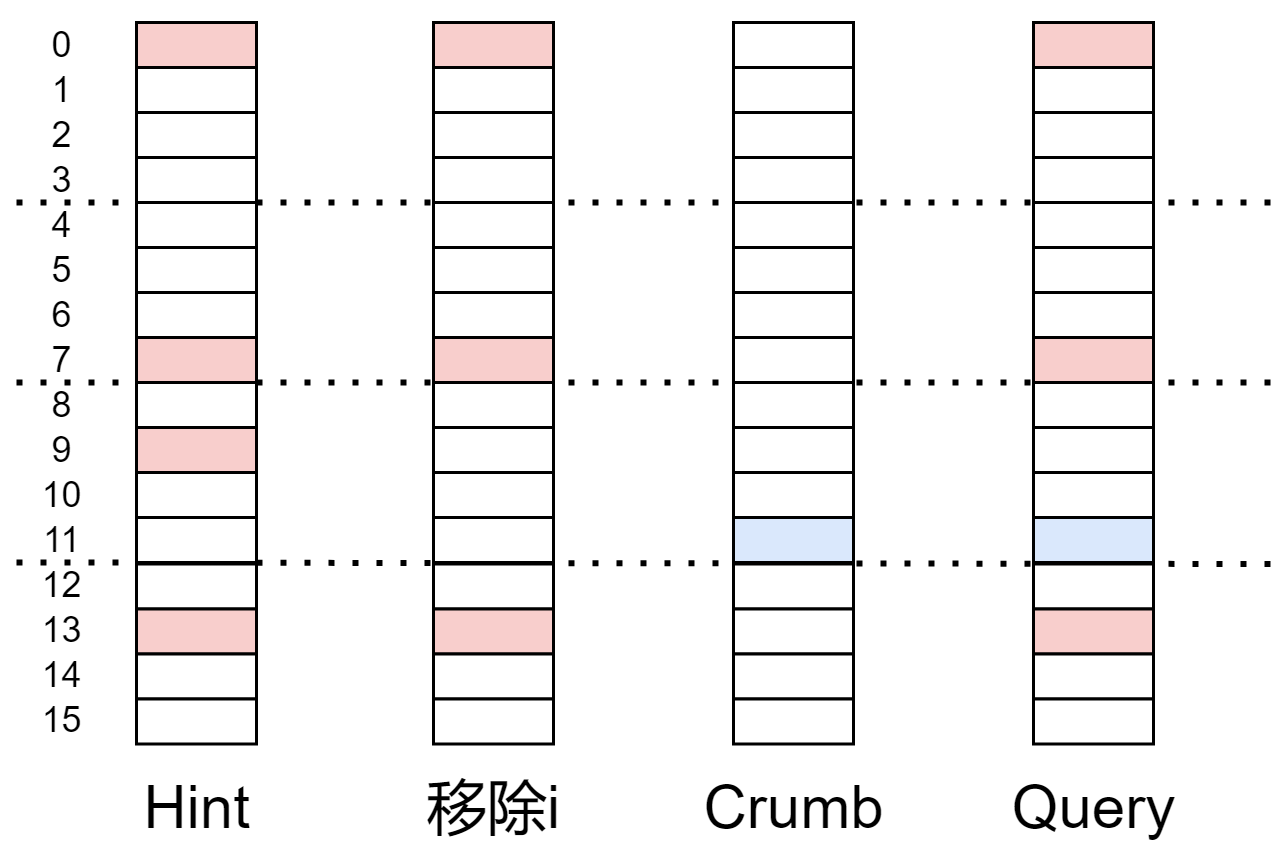
\includegraphics[width=0.8\linewidth]{figure/sketch1.png}
        \caption{查询构造} \label{fig:query-a}
    \end{subfigure}%
    \hspace*{\fill}   % maximize separation between the subfigures
    \begin{subfigure}{0.5\textwidth}
        \centering
        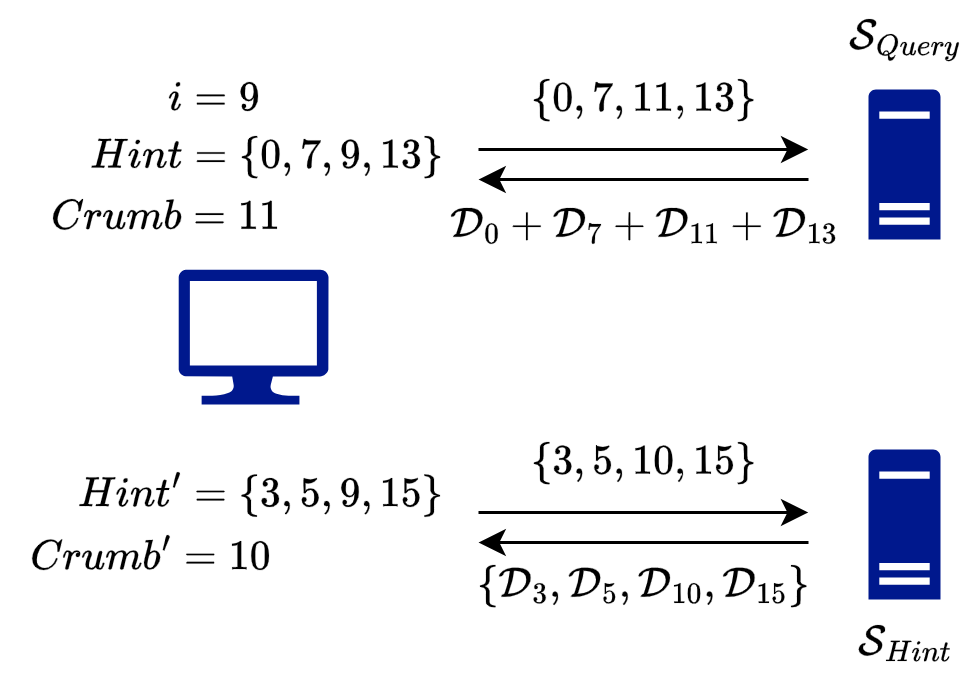
\includegraphics[width=0.8\linewidth]{figure/sketch2.png}
        \caption{查询流程} \label{fig:query-b}
    \end{subfigure}%
    \caption{一次查询的示例}
    \label{fig:query}
\end{figure}

具体来说,当客户端查询记录 $\db_\dbidx$ 时,它首先找到一个包含 $\dbidx$ 的集合 $S$。在从集合中找到 $\dbidx$ 后(由于集合划分的性质,$\dbidx$应该落在块 $\blockidx = \lfloor \dbidx/\sqrt{\dbsize} \rfloor$ 中),它会在块 $\blockidx$ 中找到一个 Crumb $\crumb=(\crumbvalue, \crumboffset)$,并将$S$中第 $\blockidx$ 块对应的偏移替换为 $\crumboffset$ 。这个过程如图 \ref{fig:query} 所示。数据库包含$\dbsize=16$条记录,并被划分为$\sqrt{\dbsize}=4$个区块。 \hyperref[fig:query-a]{a)} $Hint$包含每个块中的一个元素(图中标记为红色)。客户端希望查询记录$\dbidx=9$,该记录位于第三个块。该索引从集合中移除(在第二列中显示),第三个块中的一个Crumb被添加了到集合中(第三列和第四列标记为蓝色)。 \hyperref[fig:query-b]{b)} Query服务器以集合的校验值作为响应。客户端生成一个新的Hint集合以更新Hint和Crumb。Hint服务器以单条记录作为响应。为展示清晰起见,索引在此处以实际值表示。在真实的协议中索引在块中以偏移量表示。

用于替换的Crumb不会影响客户端计算答案。每个Crumb仅包含一个简单的记录,因此可以排除Crumb的贡献来计算真实答案。假设$\answer$是来自服务器的答案,$\crumbvalue$是所用Crumb的值,客户端计算$\answer \coloneqq \answer - \crumbvalue$。最后,客户端可以按照原本协议中的方式利用$\answer$重构记录$\db_\dbidx$。

Crumb掩盖了客户端想要查询的位置。客户端发送给服务器的集合现在由每个块中的一个元素组成,与查询的索引$\dbidx$完全无关。我们的构造保持了亚线性效率:在离线阶段,客户端接收到大小为$\recordsize\hintcount$的Hint,这些信息由服务器在$O_\lambda(\recordsize\sqrt{\dbsize}\hintcount)$时间内计算。假设$\hintcount\coloneqq \Theta_\lambda(\sqrt{\dbsize})$,当这一计算均摊在$\querycount\coloneqq\Theta_\lambda(\sqrt{\dbsize})$次在线查询上时,每次查询的通信开销为$O(\recordsize\sqrt{\dbsize})$,计算开销为$O_\lambda(\recordsize\sqrt{\dbsize})$。

\subsection{Hint的获取与更新}
Hint的获取与更新也是离线-在线PIR方案中的关键环节。有几个显然的要点,我们在设计方案时必须考虑到:
\begin{itemize}
    \item 每条记录都需要至少在某一个Hint集合内,否则,在在线阶段查询该记录将无法实现。
    \item 方案必须支持超过一定数量的在线查询,以将昂贵的离线成本分摊到这些在线查询上。
    \item 客户端不能重复使用一个Hint,否则服务器通过对比这些Hint就能获得关于查询索引的信息。因此,Hint在一次使用后必须被丢弃。
\end{itemize}

离线阶段的Hint和Crumb的获取并不困难的。鉴于服务器$\hintserver$是半诚实的,所有Hint都可以从客户端提供的一个PRF密钥中生成,服务器计算相应的校验值后发送给客户端。Crumb也可以通过相同的方式获取。

在线阶段的Hint和Crumb更新则需要更复杂的交互。在原本的协议中,更新是通过客户端生成一个包含查询索引$\dbidx$的新集合,并与服务器$\hintserver$交互以获取该集合的Hint来完成的。这一过程也需要隐藏$\dbidx$。理所应当地,我们会想要使用与查询类似的手段,用一个Crumb来掩盖住$\dbidx$。然而,在我们的协议中,Crumb就是从$\hintserver$获取的,不能再用于保护向$\hintserver$发送的请求。否则,$\hintserver$可以通过比较查询和Crumb,得知哪个块被Crumb替换了。

为了解决这一矛盾,我们采用一种不同于查询的方案来更新Hint。客户端仍然生成一个包含查询索引$\dbidx$的新集合$S'$,但是选择一个随机的索引$j$来替换块$\blockidx$中的$\dbidx$。当然,如果$\hintserver$仅以一个校验值响应查询,客户端将无法获知$\db_{j}$是什么,也就没有办法获得原集合$S'$对应的校验值。为了使客户端能够将协议进行下去,$\hintserver$必须直接将收到的查询中包含的 $\sqrt{\dbsize}$ 条记录全部发送给客户端。客户端则通过这$\sqrt{\dbsize}$条记录与之前查询得到的$\db_\dbidx$更新Hint,并使用$\db_{j}$来更新用掉的Crumb。采用这种Hint和Crumb更新方案后,我们的方案现在能够支持多项式数量的查询,这与最近在文献 \cite{C:LazPap23} 中所达成的进展一致。关于正确性的讨论将延后到第 \ref{sec:analysis} 节。完整的协议如下:

% \begin{algorithm}
    \begin{mdframed}
        \centering
        \textbf{两服务器协议}

        \raggedright
        \paragraph{符号约定:} 协议包含一个客户端 $\client$,一台Query服务器 $\queryserver$ 与一台Hint服务器 $\hintserver$。单个Hint由元祖:$\hint=(\setkey,\sumhint)$构成。单个Crumb包含了一个偏移量和一条记录值 $\crumb=(\crumboffset,\crumbvalue)$。$fk_{key}:\{0,1\}^\lambda \to \{0,1\}^\lambda$ 是一个能将单一PRF密钥映射为多个PRF密钥的PRF函数, $f_{\setkey}: [\sqrt{\dbsize}]\to [\sqrt{\dbsize}]$ 是一个将块序号转化为偏移量的PRF,  $Eval(\setkey,\dbidx) \coloneqq f_{\setkey}(\dbidx)\oplus \shift + \dbidx\cdot\sqrt{\dbsize}$ 与 $Expand$ 密钥 $\setkey$ 标识计算密钥对应的集合内元素 $\{Eval(sk,j) \mid j\in[\sqrt{\dbsize}]\}$. 假设 $\dbidx$ 是需要查询的索引。 在离线阶段,总共生成 $\hintcount$ 个 Hint.

        \paragraph{离线阶段:}
        \begin{itemize}
            \item \textbf{Setup:} $\client$ 生成一个PRF密钥 $mk\in\{0,1\}^\lambda$,将本地的Hint存储初始化为 $\hint_j\coloneqq(fk_{mk}(j),0), j\in [\hintcount]$,Crumb存储初始化为 $\crumb_j\coloneqq (\bot,\bot), j\in [\sqrt{\dbsize}]$。 $\client$ 将 $mk$ 发送给 $\hintserver$.
            \item \textbf{Hint:}
                  \begin{itemize}
                      \item $\hintserver$ 将 $mk$ 展开为PRF密钥 $\setkey_j=fk_{mk}(j), j\in[\hintcount]$ 。它将这些密钥进一步$Expand$为集合 $S_j, j\in[\hintcount]$。
                      \item $\hintserver$ 为每个集合计算校验值 $\sumhint_j\coloneqq \sum_{k\in [\sqrt{\dbsize}]}\db_{S_{j}[k]}, j\in[\hintcount]$ 。$\hintserver$将这些校验值发送给 $\client$。
                      \item 在第 $j$ 个 $\sqrt{\dbsize}$ 大小的块 ($j\in[\sqrt{N}]$) 内, $\hintserver$ 随机选取一个偏移量 $\crumboffset_j\leftarrow [\sqrt{N}]$ 及其对应的记录值 $\crumbvalue_j$ 作为Crumb。它将这些Crumb $\crumb_j \coloneqq  (\crumboffset_j, \crumbvalue_j), j\in [\sqrt{\dbsize}]$ 发送给 $\client$。 $\client$ 接受并储存这些Crumb。
                  \end{itemize}
        \end{itemize}
        \paragraph{在线阶段:}
        \begin{itemize}
            \item \textbf{Query ($\queryserver$):}
                  \begin{itemize}
                      \item 记 $\dbidx$ 所在的块为 $\blockidx\coloneqq \lfloor \dbidx/\sqrt{\dbsize}\rfloor$。 $\client$ 在存储中找到一个Hint $\hint_\hintidx = (\setkey_\hintidx,\sumhint_\hintidx)$,满足条件 $f_{\setkey_\hintidx}(\blockidx) = \dbidx-\sqrt{\dbsize}\cdot \blockidx$。如果没有这样的Hint,$\client$ 终止查询并输出 $\bot$.
                      \item $\client$ 将 $\setkey_\hintidx$ $Expand$ 为集合 $S$。$\client$ 找到 $\blockidx$ 的 Crumb $\crumb_\blockidx=(\crumboffset_\blockidx, \crumbvalue_\blockidx)$,将 $S[\blockidx]$ 替换为Crumb偏移量 $\crumboffset_\blockidx$。  $\client$ 将 $S$  发送给 $\queryserver$.
                  \end{itemize}
            \item \textbf{Answer ($\queryserver$):} $\queryserver$ 计算校验值 $\sumanswer\coloneqq \sum_{k\in [\sqrt{\dbsize}]}\db_{S[k]}$ 。$\queryserver$ 将 $\sumanswer$  发送给 $\client$.
            \item \textbf{Reconstruct:} $\client$ 重构出记录 $\db_\dbidx \coloneqq  \sumhint_\hintidx-(\sumanswer-\crumbvalue_\blockidx)$。  $\client$ 输出 $\db_\dbidx$。
            \item \textbf{Query ($\hintserver$):}
                  \begin{itemize}
                      \item $\client$ 生成PRF密钥 $\setkey'$ 使得 $f_{\setkey'}(\blockidx) = \dbidx-\sqrt{\dbsize}\cdot \blockidx$。 .
                      \item $\client$ 将 $\setkey'$ $Expand$ 为集合 $S'$。$\client$ 将 $S'[\blockidx]$ 替换为随机偏移 $\crumboffset' \leftarrow [\sqrt{\dbsize}]$. $\client$ 将 $S'$ 发送给 $\hintserver$.
                  \end{itemize}
            \item \textbf{Answer ($\hintserver$):} $\hintserver$ 直接将 $\sqrt{\dbsize}$ 条记录 $\db_{S'[j]}, j\in [\sqrt{\dbsize}]$ 发送给 $\client$。
            \item \textbf{Refresh:} $\client$ 将Crumb更新为 $\crumb_\blockidx \coloneqq  (\crumboffset', \db_{S'[\blockidx]})$,将Hint更新为 $\hint_\hintidx \coloneqq  (\setkey',\db_\dbidx + \sum_{k\in [\sqrt{\dbsize}],k\neq \blockidx}\db_{S'[k]}, )$
        \end{itemize}
    \end{mdframed}
    \label{fig:two-server}
% \end{algorithm}
\section{可验证的PIR}
\label{sec:verification}
在本节中,我们描述了一种将可验证性嵌入到PIR方案中的技术。我们首先正式提出可验证离线-在线PIR的定义,该概念扩展了先前定义的离线-在线PIR。

\begin{definition}[可验证离线-在线PIR]
    一个可验证离线-在线PIR方案$\Pi$允许客户端从数据库$\db$中检索记录$\db_\dbidx$,而不向$\servercount$个服务器中任意一个泄露索引$\dbidx$,同时确保结果的完整性。该方案包含算法组$\Pi = (Setup, Hint, Query, Answer, Reconstruct, Refresh)$:
    \begin{center}
        离线阶段:
        \begin{itemize}[leftmargin=*]
            \item $Setup(1^\lambda,\dbsize) \rightarrow \query_\hint$:给定数据库大小$\dbsize$和安全参数$\lambda$,生成Hint查询$\query_\hint$。
            \item $Hint(\db, \query_\hint) \rightarrow \hint$:根据数据库$\db$和Hint查询$\query_\hint$ 生成Hint $\hint$。
        \end{itemize}
        在线阶段:
        \begin{itemize}
            \item $Query(\hint, \dbidx) \rightarrow (\query, \clientstate)$:根据Hint~$\hint$和要查询的索引$\dbidx$生成查询$\query$。注意,查询$\query$可能由多个子查询组成。客户端生成并保存一个私有状态$\clientstate$。
            \item $Answer(\db, \query) \rightarrow \answer$:根据查询$\query$生成响应$\answer$。
            \item $Reconstruct(\clientstate, \hint, \answer) \rightarrow \{\db_\dbidx, \bot\}$:根据响应$\answer$,借助Hint~$\hint$和私有状态$\clientstate$重建记录$\db_\dbidx$,或拒绝响应并输出 $\bot$。
            \item $Refresh(\clientstate, \hint, \answer) \rightarrow \hint$:根据响应$\answer$和私有状态$\clientstate$更新Hint~$\hint$。
        \end{itemize}
    \end{center}
    在两服务器($\servercount$=2)时,我们假设Query服务器是恶意的,而Hint服务器是半诚实的。先前的工作 \cite{APIR} 采用了类似的设置,但它们不要求客户端知道哪个服务器是半诚实的。正确的数据库定义为Hint算法 $Hint$ 接受的数据库。在单服务器设置($\servercount=1$)中,正确的数据库由数据所有者提供的摘要定义。该方案应满足以下属性:

    \begin{itemize}
        \item \textbf{正确性}:给定安全参数$\lambda$,任意数据库$\db$和索引$\dbidx$以及任意多项式数量的查询索引序列$\{\dbidx_0,\dbidx_1, \dots\}$,如果服务器和客户端诚实地遵循$\Pi$,则客户端输出$\{\db_{\dbidx_0},\db_{\dbidx_1}, \dots\}$的概率为$1-negl(\lambda)$。
        \item \textbf{完整性}:给定安全参数$\lambda$,任意数据库$\db$和索引$\dbidx$,任意概率多项式时间敌手 $\adversary$作为服务器之一与客户端交互时,客户端重构出错误记录$\widehat{\db_\dbidx} \neq \db_\dbidx$的概率为 $negl(\lambda)$。
        \item \textbf{隐私性(针对选择性失败攻击)}:该属性在定义 \ref{def:privacy-sfa} 中给出。
    \end{itemize}
\end{definition}
\subsection{一种常用于多方安全计算的验证方案}
在多方安全计算协议中,函数 $m = f(x)$ 的计算通常是由一个相关量 $n = g(x) = \alpha f(x)$ 的验证的。其中, $\alpha \in \recordfield$ 代表一个隐藏的系数。验证过程检查是否有 $m\alpha = n$。多方安全计算的性质保障了参与者无法知晓他们计算出的值。诚实的参与者总是能通过此验证,而如果$\recordfield$足够大,不诚实的计算通过验证的概率非常小。

\subsection{验证方案在PIR中的应用}

在我们的协议中,我们采用类似的方法来验证$\queryanswer$的真实性。

在第 \ref{sec:construction} 节中的构造中,客户端最初从服务器获取了一些Hint。我们选择在每个Hint中包含一个额外的校验值,以使客户端能够进行后续的答案验证。升级后的Hint中的校验值包含两个部分:和校验$\sumhint$和随机校验$\randomhint$。对于一个特定集合$S = \{x_j \mid j\in [\setsize]\}$,一组随机数 $SR\coloneqq \{r_j \mid j\in [\setsize]\}$,$\sumhint, \randomhint$ 定义为如下:

$$
    \begin{array}{l}
        \sumhint \coloneqq  \sum_{j \in [\setsize]} \db_{x_j}, \\
        \randomhint \coloneqq  \sum_{j \in [\setsize]} r_j\cdot \db_{x_j}
    \end{array}
$$

查询被分为两个不同的部分:和查询$\sumquery$和随机查询$\randomquery$。假设$x_\dbidx$是查询的索引。$\sumquery$和$\randomquery$的定义如下:

$$
    \begin{array}{l}
        \sumquery \coloneqq  S \setminus \{x_\dbidx\}, \\
        \randomquery \coloneqq  SR \setminus \{r_\dbidx\}
    \end{array}
$$

在接收到这两个查询后,Query服务器计算答案$\sumanswer$和$\randomanswer$:

$$
    \begin{array}{l}
        \sumanswer \coloneqq  \sum_{j \in [s-1]} \db_{\sumquery_j}, \\
        \randomanswer \coloneqq  \sum_{j \in [s-1]} \randomquery_j\cdot \db_{\sumquery_j}
    \end{array}
$$

Query服务器将答案发送给客户端,客户端重构记录$\db_{x_\dbidx} \coloneqq \sumhint-\sumanswer$,通过以下条件来验证答案:

$$
    \randomhint-\randomanswer = r_\dbidx \cdot (\sumhint-\sumanswer)
$$

如果Query服务器如实作答,则等式的左边等于$r_{\dbidx} \cdot \db_{x_\dbidx}$。由于$\sumhint - \sumanswer = \db_{x_\dbidx}$,等式应成立。如果验证未通过,客户端输出 $\bot$。

在我们的框架中,我们进一步采用第 \ref{sec:construction} 节中讨论的利用PRF压缩集合的策略来提高空间效率。集合 $S$ 可以使用密钥$\setkey$通过一个PRF展开。集合$SR$ 可以通过另一个PRF展开:$fr_{\randomset}: [\sqrt{\dbsize}] \to \recordfield$。因此,集合 SR 也可以用一个短密钥$\randomset$来表示。

$$
    \randomset \to SR = \{fr_{\randomset}(j) \mid j\in[\sqrt{\dbsize}]\}
$$

稍稍滥用符号,我们使用 $Eval(\randomset, j)$ 作为 $fr_{\randomset}(j)$ 的简写。

与索引集合一致,这一随机数组成的集合$SR$中被删去元素的位置必然在包含查询索引$\dbidx$的块中。在半诚实方案中,一个随机Crumb($\crumb$)替换了被删去的索引,从而隐藏了$\dbidx$所在的块。同样,在验证方案中,一个随机元素$r \leftarrow \recordfield$可以用于隐藏$SR$中被删去删除的元素。具体来说,令$\blockidx \coloneqq \lfloor \dbidx /\sqrt{\dbsize} \rfloor$为包含查询索引$\dbidx$的块,客户端从$\recordfield$中采样$r \leftarrow \recordfield$,并将$SR[\blockidx]$替换为$r$。在客户端接收到响应$\randomanswer$后,它可以移除Crumb值的贡献($\crumbvalue$)并更新$\randomanswer$,即:
$$\randomanswer \coloneqq \randomanswer - r\cdot \crumbvalue$$
随后,客户端通过检查
$$\randomhint-\randomanswer = Eval(\randomset,\blockidx)\cdot \db_{\dbidx}$$
来执行验证。如果验证失败,客户端输出$\bot$。

我们在下图中展示了我们的双服务器可验证PIR方案,其中验证过程以蓝色突出显示。

% \begin{figure*}
    \begin{mdframed}
        \centering
        \textbf{可验证两服务器协议}

        \raggedright
        \paragraph{符号约定:} 协议包含一个客户端 $\client$,一台Query服务器 $\queryserver$ 与一台Hint服务器 $\hintserver$。单个Hint由元组:$\hint=(\setkey,\sumhint,\bluetext{\randomset,\randomhint})$构成。单个Crumb包含了一个偏移量和一条记录值 $\crumb=(\crumboffset,\crumbvalue)$。$fk_{key}:\{0,1\}^\lambda \to \{0,1\}^\lambda$ 是一个能将单一PRF密钥映射为多个PRF密钥的PRF函数, $f_{\setkey}: [\sqrt{\dbsize}]\to [\sqrt{\dbsize}]$ 是一个将块序号转化为偏移量的PRF, \bluetext{$fr_{\randomset}: [\sqrt{\dbsize}]\to \recordfield$ 是一个将块序号转化为 $\recordfield$上的随机元素的PRF。} $Eval(\setkey,\dbidx) \coloneqq f_{\setkey}(\dbidx)\oplus \shift + \dbidx\cdot\sqrt{\dbsize}$ 与 $Expand$ 密钥 $\setkey$ 标识计算密钥对应的集合内元素 $\{Eval(sk,j) \mid j\in[\sqrt{\dbsize}]\}$。 \bluetext{$Eval(\randomset,\dbidx) \coloneqq fr_{\randomset}(\dbidx)$ 与 $Expand$ 密钥 $\randomset$ 表示计算集合元素 $\{Eval(sr,j) \mid j\in[\sqrt{\dbsize}]\}$。} 假设 $\dbidx$ 是需要查询的索引。 在离线阶段,总共生成 $\hintcount$ 个 Hint。

        \paragraph{离线阶段:}
        \begin{itemize}
            \item \textbf{Setup:} $\client$ 生成一个PRF密钥 $mk\in\{0,1\}^\lambda$,将本地的Hint存储初始化为 $\hint_j\coloneqq(fk_{mk}(j),0,\bluetext{fk_{mk}(j+\hintcount),0}), j\in [\hintcount]$,Crumb存储初始化为 $\crumb_j\coloneqq (\bot,\bot), j\in [\sqrt{\dbsize}]$。 $\client$ 将 $mk$ 发送给 $\hintserver$.
            \item \textbf{Hint:}
                  \begin{itemize}
                      \item $\hintserver$ 将 $mk$ 展开为PRF密钥 $\setkey_j=fk_{mk}(j), j\in[\hintcount]$ \bluetext{与 $\randomset_j=fk_{mk}(j+\hintcount), j\in[\hintcount]$}。它将这些密钥进一步$Expand$为集合 $S_j, j\in[\hintcount]$ \bluetext{与 $SR_j, j\in[\hintcount]$}.
                      \item $\hintserver$ 为每个集合计算校验值 $\sumhint_j\coloneqq \sum_{k\in [\sqrt{\dbsize}]}\db_{S_{j}[k]}, j\in[\hintcount]$ \bluetext{与 $\randomhint_j\coloneqq \sum_{k\in [\sqrt{\dbsize}]}\db_{S_{j}[k]}\cdot SR_{j}[k], j\in[\hintcount]$}。$\hintserver$将这些校验值发送给 $\client$.
                      \item 在第 $j$ 个 $\sqrt{\dbsize}$ 大小的块 ($j\in[\sqrt{N}]$) 内, $\hintserver$ 随机选取一个偏移量 $\crumboffset_j\leftarrow [\sqrt{N}]$ 及其对应的记录值 $\crumbvalue_j$ 作为Crumb。它将这些Crumb $\crumb_j \coloneqq  (\crumboffset_j, \crumbvalue_j), j\in [\sqrt{\dbsize}]$ 发送给 $\client$。 $\client$ 接受并储存这些Crumb。
                  \end{itemize}
        \end{itemize}
        \paragraph{在线阶段:}
        \begin{itemize}
            \item \textbf{Query ($\queryserver$):}
                  \begin{itemize}
                      \item 记 $\dbidx$ 所在的块为 $\blockidx\coloneqq \lfloor \dbidx/\sqrt{\dbsize}\rfloor$。 $\client$ 在存储中找到一个Hint $\hint_\hintidx = (\setkey_\hintidx,\sumhint_\hintidx,\bluetext{\randomset_\hintidx,\randomhint_\hintidx})$,满足条件 $f_{\setkey_\hintidx}(\blockidx) = \dbidx-\sqrt{\dbsize}\cdot \blockidx$。如果没有这样的Hint,$\client$ 终止查询并输出 $\bot$。
                      \item $\client$ 将 $\setkey_\hintidx$ $Expand$ 为集合 $S$。$\client$ 找到 $\blockidx$ 的 Crumb $\crumb_\blockidx=(\crumboffset_\blockidx, \crumbvalue_\blockidx)$,将 $S[\blockidx]$ 替换为Crumb偏移量 $\crumboffset_\blockidx$。 \bluetext{$\client$ 将 $\randomset_\hintidx$ $Expand$ 为集合 $SR$,并将 $SR[\blockidx]$ 替换为一随机元素 $r\leftarrow \recordfield$。} $\client$ 将 $S$ \bluetext{与 $SR$} 发送给 $\queryserver$。
                  \end{itemize}
            \item \textbf{Answer ($\queryserver$):} $\queryserver$ 计算校验值 $\sumanswer\coloneqq \sum_{k\in [\sqrt{\dbsize}]}\db_{S[k]}$ \bluetext{与 $\randomanswer\coloneqq \sum_{k\in [\sqrt{\dbsize}]}\db_{S[k]}\cdot SR[k]$}。$\queryserver$ 将 $\sumanswer$ \bluetext{与 $\randomanswer$} 发送给 $\client$.
            \item \textbf{Reconstruct:} $\client$ 重构出记录 $\db_\dbidx \coloneqq  \sumhint_\hintidx-(\sumanswer-\crumbvalue_\blockidx)$。 \bluetext{$\client$ 验证是否有 $\randomhint_\hintidx-(\randomanswer-r\cdot \crumbvalue_\blockidx) = Eval(\randomset_\hintidx, \blockidx)\cdot \db_\dbidx$。如果验证失败,$\client$ 输出 $\bot$。否则, } $\client$ 输出 $\db_\dbidx$。
            \item \textbf{Query ($\hintserver$):}
                  \begin{itemize}
                      \item $\client$ 生成PRF密钥 $\setkey'$ 使得 $f_{\setkey'}(\blockidx) = \dbidx-\sqrt{\dbsize}\cdot \blockidx$。 \bluetext{$\client$ 生成PRF密钥 $\randomset'$}.
                      \item $\client$ 将 $\setkey'$ $Expand$ 为集合 $S'$, \bluetext{将 $\randomset'$ $Expand$ 为集合 $SR'$}。$\client$ 将 $S'[\blockidx]$ 替换为随机偏移 $\crumboffset' \leftarrow [\sqrt{\dbsize}]$. $\client$ 将 $S'$ 发送给 $\hintserver$.
                  \end{itemize}
            \item \textbf{Answer ($\hintserver$):} $\hintserver$ 直接将 $\sqrt{\dbsize}$ 条记录 $\db_{S'[j]}, j\in [\sqrt{\dbsize}]$ 发送给 $\client$。
            \item \textbf{Refresh:} $\client$ 将Crumb更新为 $\crumb_\blockidx \coloneqq  (\crumboffset', \db_{S'[\blockidx]})$,将Hint更新为 $\hint_\hintidx \coloneqq  (\setkey',\db_\dbidx + \sum_{k\in [\sqrt{\dbsize}],k\neq \blockidx}\db_{S'[k]}, \bluetext{\randomset', SR[l]\cdot \db_\dbidx + \sum_{k\in [\sqrt{\dbsize}],k\neq \blockidx}SR[k]\cdot \db_{S'[k]}})$
        \end{itemize}
    \end{mdframed}
    \label{fig:two-server-verify}
% \end{figure*}

% 我们提出了以下关于安全性和效率的定理:

% \begin{theorem}
%     \label{thm:1}
%     图 \ref{fig:two-server-verify} 中描述的方案是一个双服务器可验证的离线-在线PIR方案。设 $\alpha(\lambda)$ 为任意超常数函数,即$\alpha(\lambda)$ = $\omega(1)$。假设数据库索引大小为$O(1)$,PRF密钥大小为$O_\lambda(1)$。在一个包含$\dbsize$条记录、每条大小为$\recordsize$的数据库上,存储$\hintcount = \magictotal$个Hint,该方案的效率如下:
    
%     \noindent 在离线阶段:
%     \begin{itemize}[itemsep=0em]
%         \item 通信量为$O_\lambda(1)$上传,$2\recordsize\hintcount + \recordsize\sqrt{\dbsize} + O(\sqrt{\dbsize})$下载。
%         \item 客户端计算复杂度为$O_\lambda(\hintcount)$,服务器计算复杂度为$O_\lambda(\hintcount) + O(\recordsize\sqrt{\dbsize}\hintcount)$。
%     \end{itemize}
%     在在线阶段:
%     \begin{itemize}[itemsep=0em]
%         \item 向Query服务器通信量为:$\recordsize\sqrt{\dbsize} + O(\sqrt{\dbsize})$上传,$2\recordsize$下载。
%         \item 向Hint服务器通信量为:$O(\sqrt{\dbsize})$上传,$\recordsize\sqrt{\dbsize}$下载。
%         \item 客户端计算复杂度为$O_\lambda(\sqrt{\dbsize}) + O(\recordsize\sqrt{\dbsize})$,服务器计算复杂度为$O(\recordsize\sqrt{\dbsize})$。
%         \item 支持多项式数量的查询。
%     \end{itemize}
% \end{theorem}

% \paragraph{恶意的Hint服务器}
% 当Hint服务器是恶意的时,该协议是不安全的。在附录 \ref{appendix:hint-server} 中提供了详细的解释和示例。
\section{单服务器模型}
这一节中,我们将前文方案修改为单服务器可验证的PIR。我们假设数据所有者将数据库外包给单个服务器,并生成一个数据库摘要。客户端可以使用此摘要对查询结果进行验证。为实现这一修改,有两个主要问题需要解决:
\begin{enumerate}
    \item \textbf{获取Hint:} 在双服务器设置中,Hint服务器负责向客户端提供Hint。在单服务器设定中,我们不能让Query服务器来完成这一任务。如果在线查询的服务器同时也知道离线生成的Hint,它可以通过比对Hint和查询来推断客户端正在查询的索引。
    \item \textbf{更新Hint:} 为了让客户端能够执行多次查询,方案必须支持Hint更新。然而,原本的方案中,查询与Hint更新是由两台不同的服务器执行的。
\end{enumerate}

此外,还需要考虑客户端如何确保托管给不可信服务器的数据库的正确性。我们将在以下部分中解决上述问题。

\subsection{将协议修改为单服务器}

\paragraph{使用备用更新Hint}
为了在在线阶段更新Hint,我们采用了备用Hint的做法 \cite{EC:CorHenKog22}。客户端在离线阶段获取额外的Hint。这些备用Hint用于更新在线阶段消耗的Hint。

我们将Hint分为两类:主Hint和备用Hint。客户端获取$\hintcount_1$个主Hint。除此之外,客户端还为每个块获取$\hintcount_2$个备用Hint。块$\blockidx$的备用Hint在第$\blockidx$块中留空。换句话说,块$\blockidx$的备用Hint中不包含块$\blockidx$中的索引。客户端按照双服务器方案使用主Hint向服务器发出查询。一旦完成对块$\blockidx$中某个索引的查询,客户端获取块$\blockidx$的备用Hint,将查询的索引加入该备用Hint中,填补块$\blockidx$中缺失的部分并更新校验信息。这一过程完成后,该备用Hint转化为主Hint。

Crumb也遵循类似的模式。客户端在离线阶段为每个块保留$\hintcount_2$个备用Crumb,并在查询后从备用中获取一个对应块的新Crumb。

可以证明,若为每个块分配了$3\magicnumber$个备用Hint和Crumb,该方案能够让客户端在一个离线阶段后以极高的概率成功执行至少$\magictotal$次查询。在此之后,双方重新运行离线阶段以补充Hint与Crumb。

\paragraph{通过流式传输数据库获取Hint}
从现有工作来看,在单服务器环境下中,离线获取Hint可以通过两种方式实现:(i)  使用同态加密来计算Hint\cite{EC:CorHenKog22},(ii) 将整个数据库流式传输到客户端\cite{CCS:PatPerYeo18, Piano}。

我们采用了后者,因为它在实际运行中更为高效。数据库按前文所述方法划分$\sqrt{\dbsize}$个块。客户端首先生成所有需要的Hint集合,并从服务器请求$\sqrt{\dbsize}$个块中的一个,更新所有本地Hint。具体来说,当处理第$j$个块时,对于具有校验值$\hint_\hintidx$和PRF密钥$\setkey_\hintidx$的Hint,客户端计算$\hint_\hintidx \coloneqq \hint_\hintidx+\db_{Eval(\setkey_\hintidx,j)}$。如果Hint不应该包含该块中的任何索引(它是一个此块的备用Hint),则跳过该Hint。所有Hint更新完成后,客户端丢弃这个块并从服务器获取一个新块。

\paragraph{引入验证}
单服务器与双服务器协议唯一的不同点是,利用流式传输的方式获取Hint时,我们要求数据库所有者提供数据库的摘要,这与前人的工作 \cite{APIR} 中的假设一致。该摘要可以通过签名发布在区块链等可信平台上。在执行在线查询之前,客户端需要根据此摘要验证流式传输的数据库,以确保数据库内容的真实性和完整性。

到目前为止,我们已经解决了将双服务器可验证PIR方案转换为单服务器环境所面临的主要问题。但在完整给出我们的单服务器构造之前,还有一些重要的辅助手段需要介绍:
\begin{itemize}
    \item \textbf{支持$\querycount = \Omega(\sqrt{\dbsize})$次查询就能支持多项式数量的查询:} 在进行$\querycount$次查询后,协议双方可以重新执行离线阶段。只要方案能在$O_\lambda(\recordsize\dbsize)$时间内完成离线阶段,客户端将这一复杂度均摊到$\querycount$次查询上时,查询的复杂度就是亚线性的。这一离线-在线的循环过程可以支持多项式数量的查询。

    \item \textbf{查询不会重复:} 不失普遍性地,我们可以假设在$\querycount$ 次查询中没有重复查询。我们可以令客户端使用额外$\Theta(\recordsize \querycount)$的存储空间缓存最近的$\querycount$个查询结果。如果客户端需要提出一个重复查询,它可以随机查询一个未查询过的数据库记录,并从缓存结果中检索需要的信息。

    \item \textbf{查询的分布是均匀的:} 不失普遍性地,我们假设查询的索引在数据库中是均匀的。数据库所有者可以根据伪随机置换(PRP)密钥对数据库条目进行洗牌。我们还可以假设查询索引是在不知道这一置换密钥的情况下选择的。由于我们先前假设了查询中没有重复,每个查询索引将被映射到洗牌后数据库中的随机索引,并落入一个随机块。
\end{itemize}

总结上述内容,我们在下图中展示了我们的单服务器可验证PIR方案,其中验证过程以蓝色标记突出显示。

% \begin{figure*}
    \begin{mdframed}
    \centering
    \textbf{可验证单服务器协议}
        \raggedright
        \paragraph{符号约定:} 协议包含一个客户端 $\client$ 与一台Query服务器 $\queryserver$。单个Hint由元组:$\hint=(\setkey,x,\sumhint,\bluetext{\randomset,\randomhint})$构成。单个Crumb包含了一个偏移量和一条记录值 $\crumb=(\crumbvalue, \crumboffset)$。$f_{\setkey}: [\sqrt{\dbsize}]\to [\sqrt{\dbsize}]$ 是一个将块序号转化为偏移量的PRF,\bluetext{$fr_{\randomset}: [\sqrt{\dbsize}]\to \recordfield$ 是一个将块序号转化为 $\recordfield$上的随机元素的PRF。} $Eval(\setkey,\dbidx) \coloneqq f_{\setkey}(\dbidx)\oplus \shift + \dbidx\cdot\sqrt{\dbsize}$ 与 $Expand$ 密钥 $\setkey$ 标识计算密钥对应的集合内元素 $\{Eval(sk,j) \mid j\in[\sqrt{\dbsize}]\}$。 \bluetext{$Eval(\randomset,\dbidx) \coloneqq fr_{\randomset}(\dbidx)$ 与 $Expand$ 密钥 $\randomset$ 表示计算集合元素 $\{Eval(sr,j) \mid j\in[\sqrt{\dbsize}]\}$。} 假设 $\dbidx$ 是需要查询的索引。\bluetext{可信的数据库所有者 $\owner$ 计算数据库 $\db$ 的摘要 $\digest$ 并且将其发送给 $\client$。} 在离线阶段,生成 $\hintcount_1$ 个主Hint与每块 $\hintcount_2$ 个备用Hint。

        \paragraph{离线阶段:}
        \begin{itemize}
            \item \textbf{Setup:} $\client$ 生成主PRF密钥 $\setkey_j, j\in[\hintcount]$,备用PRF密钥 $\setkey_{k,j}, j\in[\lambda], k\in[\sqrt{\dbsize}]$ \bluetext{与 $\randomset_j, j\in[\hintcount]$ 及其备用密钥 $\randomset_{k,j}, j\in[\lambda], k\in[\sqrt{\dbsize}]$},将本地的主Hint存储初始化为 $\hint_j\coloneqq(\setkey_j,\bot,0,\bluetext{\randomset_j,0}), j\in[\hintcount]$,备用Hint初始化为 $\hint_{k,j}\coloneqq(\setkey_{k,j},\bot, 0,\bluetext{\randomset_{k,j},0}), j\in[\lambda], k\in[\sqrt{\dbsize}]$,Crumb存储初始化为$\crumb_{k,j} \coloneqq (\bot,\bot),j\in[\lambda], k\in[\sqrt{\dbsize}]$。
            \item \textbf{Hint:} 服务器 $\queryserver$ 将数据库 $\db$ 传输给 $\client$。\bluetext{$\client$ 初始化摘要 $\digest'$.} 当传输块 $l$ 时, $\client$ 按如下方法更新Hint:
                  \begin{itemize}
                      \item 更新主Hint: 对于所有 $j\in[\hintcount]$,$\sumhint_j \coloneqq \sumhint_j+\db_{Eval(\setkey_j, l)}$ \bluetext{以及 $\randomhint_j \coloneqq  \randomhint_j+Eval(\randomset_j, l)\cdot \db_{Eval(\setkey_j, l)}$}。
                      \item 更新不属于此块的备用Hint:对于所有 $j\in[\lambda], k\in[\sqrt{\dbsize}], k\neq l$ 的 $\sumhint_{k,j}$ \bluetext{和 $\randomhint_{k,j}$},$\sumhint_{k,j} \coloneqq  \sumhint_{k,j}+\db_{Eval(\setkey_{k,j}, l)} $ \bluetext{以及 $\randomhint_{k,j} \coloneqq  \randomhint_{k,j}+Eval(\randomset_{k,j}, l)\cdot \db_{Eval(\setkey_{k,j}, l)}$}。
                      \item 将块$l$的 Crumb $\crumb_{l,j}$ 更新为随机选择的记录值以及对应的偏移 $(\crumbvalue_{l,j}, \crumboffset_{l,j}), j\in[\lambda] $。
                      \item \bluetext{$\client$ 用块$l$的内容更新 $\digest'$。}
                      \item 完成之后,$\client$ 从储存中删除此块。
                    \end{itemize}
                \item \bluetext{$\client$ 检查是否有 $\digest = \digest'$。如果不成立, $\client$ 终止协议并输出 $\bot$。}
        \end{itemize}
        \paragraph{在线阶段:}
        \begin{itemize}
            \item \textbf{Query:}
                  \begin{itemize}
                      \item 记 $\dbidx$ 所在块为 $\blockidx\coloneqq \lfloor \dbidx/\sqrt{\dbsize}\rfloor$。 \redtext{\client 记录每一块被查询了多少次。如果块 $\blockidx$ 已经被查询了超过 $\hintcount_2$ 次, \client 随机选择一个被查询少于$\hintcount_2$ 的块中索引 $\dbidx'$ 作为查询对象,并重新运行在线阶段。} $\client$ 在存储中找到一个Hint $\hint_\hintidx = (\setkey_\hintidx,x_\hintidx,\sumhint_\hintidx,\bluetext{\randomset_\hintidx,\randomhint_\hintidx})$。这个Hint需要包含 $\dbidx$ ( $x_\hintidx=\dbidx$ 或是 $Eval(\setkey_\hintidx, \blockidx) + \sqrt{\dbsize}\cdot \blockidx = \dbidx $ 且有 $x_\hintidx = \bot \vee \lfloor x_\hintidx/\sqrt{\dbsize}\rfloor\neq \blockidx$). 如果没有这样的Hint,$\client$ 终止查询并输出 $\bot$。
                      \item $\client$ 将 $\setkey_\hintidx$ $Expand$ 为集合 $S$。如果$x_\hintidx\neq \bot$,将$S[\lfloor x_\hintidx/\sqrt{\dbsize}\rfloor]$ 替换为 $x_\hintidx$。$\client$找到一个块$\blockidx$中的Crumb $\crumb_{\blockidx, \crumbidx}=(\crumbvalue_{\blockidx, \crumbidx},\crumboffset_{\blockidx, \crumbidx})$ 并将 $S[\blockidx]$ 替换为  $\crumboffset_{\blockidx, \crumbidx}$。 \bluetext{$\client$ 将 $\randomset_\hintidx$ $Expand$ 为集合 $SR$,将 $SR[\blockidx]$ 替换为随机数 $r\leftarrow \recordfield$。} $\client$ 将 $S$ \bluetext{与 $SR$} 发送给 $\queryserver$。
                  \end{itemize}
            \item \textbf{Answer:} $\queryserver$ 计算校验值 $\sumanswer\coloneqq \sum_{k\in [\sqrt{\dbsize}]}\db_{S[k]}$ \bluetext{以及 $\randomanswer\coloneqq \sum_{k\in [\sqrt{\dbsize}]}\db_{S[k]}\cdot SR[k]$}。$\queryserver$ 将 $\sumanswer$ \bluetext{与 $\randomanswer$} 发送给 $\client$。
            \item \textbf{Reconstruct:} $\client$ 重构出记录 $\db_\dbidx \coloneqq  \sumhint_\hintidx-(\sumanswer-\crumbvalue_{\blockidx, \crumbidx})$。 \bluetext{$\client$ 验证是否有  $\randomhint_\hintidx-(\randomanswer-r\cdot \crumbvalue_{\blockidx, \crumbidx}) = Eval(\randomset_\hintidx, \blockidx)\cdot \db_\dbidx$。如果验证失败,$\client$ 输出 $\bot$。否则, } $\client$ 输出 $\db_\dbidx$。
            \item \textbf{Refresh:}
                  \begin{itemize}
                      \item $\client$ 找到一个块$\blockidx$中的未使用备用Hint $\hint_{\blockidx,j}=(\setkey_{\blockidx,j},\bot,\sumhint_{\blockidx,j},\bluetext{\randomset_{\blockidx,j},\randomhint_{\blockidx,j}})$。如果块中已经没有备用Hint了,$\client$ 直接结束$Refresh$算法。
                      \item $\client$ 更新Hint:$\hint_\hintidx \coloneqq (\setkey_{\blockidx,j}, \dbidx, \sumhint_{\blockidx,j} + \db_\dbidx, \bluetext{\randomset_{\blockidx,j},\randomhint_{\blockidx,j}+Eval(\randomset_{\blockidx,j},\blockidx)\cdot \db_\dbidx})$.
                  \end{itemize}
        \end{itemize}
    \end{mdframed}
    % \caption{单服务器PIR协议。蓝色部分是验证过程。红色与蓝色部分都可以在半诚实模型中移除。}
    \label{fig:single-server}
% \end{figure*}

\paragraph{选择失败攻击引入的问题}
为了应对选择性失败攻击,我们希望采用更强的正确性定义,尤其是允许敌手选择被查询的索引。然而,单服务器方案无法支持这种情况,因为敌手可能会使查询在不同的块之间不平衡,从而导致正确性失效,这会阻碍隐私保护。为解决这一问题,我们在单服务器协议中引入了一些额外措施(以红色标记),即当客户端无法查询给定的索引时,会随机查询一个索引。

我们认为:(i) 这并不与正确性的定义相矛盾,因为在定义中索引是在进行置换之前选择的;(ii) 该解决方案与本文的目标一致,因为报告此类失败对客户端或服务提供商没有任何好处;(iii) 该解决方案不会影响实用性,因为协议的诚实执行不受影响,并且敌手总是可以通过拒绝响应来阻止客户端检索所需的索引。

\subsection{离线处理方案的可行性}
单服务器版本的方案以及一些文献\cite{Piano, EC:CorHenKog22}中提出的构造引入了大量的离线通信。我们先前提到的另一种方案\cite{EC:CorHenKog22}使用同态加密计算Hint。该论文提出了一个基于LHE(线性同态加密)的实际方案以及一个基于FHE(全同态加密)的理论方案。我们尚不清楚如何在实践中实现FHE方案。LHE方案需要$\softO(\recordsize\sqrt{\dbsize \querycount} + \dbsize)$的离线通信。将本文的参数$\querycount=\magictotal$代入,结果为$\softO(\recordsize\dbsize^{3/4} + \dbsize)$,且有较大的对数和常数因子。此外,该方案需要$\softO(\dbsize^{3/4}+\recordsize\sqrt{\dbsize})$的在线通信和计算。与本文$\recordsize\dbsize$离线通信相比,当数据库的记录数超过 $\lambda^6 \approx 2^{42}$ 时,可能会有一定的优势。此时若每条记录的大小为$\recordsize = \Theta(\lambda)$,数据库的大小至少为 64 TiB。并且,该方案在线查询的效率较低。

\subsection{针对在线查询的优化}
\label{sec:optimized-model}
使用备用Hint进行更新的做法也可以应用于双服务器方案。具体来说,客户端从Hint服务器获取额外的备用Hint和Crumb,从而可以和单服务器场景一样,在线查询时仅与一台服务器交互。然而,在离线阶段客户端与服务器并不需要流式传输整个数据库。只需要让客户端将PRF密钥发送给Hint服务器,采用与双服务器协议类似的离线Hint算法即可。如此,客户端可以避免与半诚实服务器进行在线交互,同时最大限度地减少离线通信。这一方案为服务提供商提供了一个实用框架。数据库所有者可以利用空闲带宽提供离线Hint获取服务,并将实时查询委托给不可信的服务器。
\section{协议分析与安全性证明}
\label{sec:analysis}

在证明中,为了简化处理,我们假设方案中的PRF是完全随机的。

\subsection{扩展至多个查询}
\label{appendix:extension-to-multiple-queries}
要证明双服务器方案可以处理多项式数量的查询,只需要证明每次查询后Hint的分布保持不变。

\begin{lemma}
\label{lemma:extension}
在离线阶段结束时,以及每次查询后,客户端的Hint$\hint$遵循相同的分布,与$\hintcount$个每个块包含一条随机记录的随机集合分布无法区分。
\end{lemma}

\begin{proof}
在离线阶段结束时,该引理的正确性直接由方案和PRF的安全性推出。在在线阶段,只需证明在每次查询过程中,消耗的Hint和更新的Hint信息遵循相同的分布。对于落在第$\blockidx$个块的查询$\dbidx$,找到的查询集合$\setkey_\hintidx$和新采样的集合$\setkey'$在除$\blockidx$之外的每个块中都是均匀随机的,而在块$\blockidx$中必然为$\dbidx$。
\end{proof}

由引理 \ref{lemma:extension},针对第一次查询的正确性证明可以扩展到后续的查询。在接下来的证明中,除非特别说明,我们假设Hint信息的分布在查询发生时不会改变,并省略了Hint的初始化、消耗和更新过程,以简化表述。

\subsection{正确性}

我们首先给出正确性的形式化定义。

\begin{definition}[双服务器方案的正确性]
给定安全参数 $\lambda$,对于任意数据库$\db$和索引$\dbidx$以及任意多项式长度的查询索引序列$\{\dbidx_0,\dbidx_1, \dots\}$,如果两台服务器和客户端都诚实地遵循协议,客户端以概率$PC_\dbidx \geq 1-\negl(\lambda)$ 输出$\db_\dbidx$。
\end{definition}

\begin{theorem}
    当$\hintcount=\magictotal$时,第 \ref{fig:two-server} 节中的协议满足正确性。
\end{theorem}

\begin{proof}
    当且仅当 $Query$ 算法中客户端找不到包含查询索引的Hint时,客户端无法检索到记录。我们证明这一事件的概率是可忽略的。首先,我们证明以下引理:

    \begin{lemma}
    \label{lemma:hint-prob}
        每个Hint包含特定索引$\dbidx$的概率为$\frac{1}{\sqrt{\dbsize}}$。
    \end{lemma}

    \begin{proof}
    每个Hint在大小为$\sqrt{\dbsize}$的每个块中包含一条随机记录。任一特定索引必然落在某个块中,并以$\frac{1}{\sqrt{\dbsize}}$的概率被选中。
    \end{proof}

    根据引理 \ref{lemma:hint-prob},客户端找不到包含查询索引的Hint的概率至多为$(1-\frac{1}{\sqrt{\dbsize}})^\hintcount$。当$\hintcount=\magictotal$时,$(1-\frac{1}{\sqrt{\dbsize}})^{\magictotal}\le \lambda^{-\alpha(\lambda)} \le \negl(\lambda)$。
\end{proof}

\begin{definition}[单服务器方案的正确性]
给定安全参数 $\lambda$,对于任意数据库$\db$和索引$\dbidx$以及任意长度不超过$\querycount=\magictotal$的查询索引序列$\{\dbidx_0,\dbidx_1, \dots\}$。如果服务器和客户端诚实地遵循协议,在一次离线阶段之后,客户端至少能以概率$PC_\dbidx \geq 1-\negl(\lambda)$输出$\db_\dbidx$。
\end{definition}

\begin{theorem}
    当每个块有$\hintcount_1=\magictotal$个主Hint和$\hintcount_2 = \backuphintcount$个备用Hint时,第 \ref{fig:single-server} 节中的协议满足正确性。
\end{theorem}

\begin{proof}
有两种情况下客户端无法获取$\dbidx$。第一种情况与双服务器方案相同。第二种情况是某个块内有超过$\hintcount_2$次查询。我们证明以下引理:

\begin{lemma}
\label{lemma:crumb-prob}
    对于$\querycount=\magictotal$次查询,落在某个块内的查询超过$\backuphintcount$次的概率关于$\lambda$是可忽略的。
\end{lemma}

\begin{proof}
    在一个块中期望的查询次数是$\magicnumber$。该概率可以通过切尔诺夫界限来限定。令$X$表示落在第一个块中的查询次数,取$\delta=2$。
$$ Pr(X \ge (1+2)\magicnumber) \le e^{-2^2\magicnumber/(2+2)} = \lambda^{-\alpha(\lambda)} $$ 
对所有块使用联合界限,该概率最多为
$$\sqrt{\dbsize}\lambda^{-\alpha(\lambda)} \le \negl(\lambda)$$
\end{proof}

单服务器的正确性直接来自于双服务器正确性的论证和引理 \ref{lemma:crumb-prob}。
\end{proof}

从现在起,我们假设 $Query$ 算法永远不会失败。这对于双服务器方案是显而易见的,因为正确性证明表明客户端可以以压倒性概率找到Hint。对于单服务器方案,我们在第 \ref{fig:single-server} 节中的协议内引入了一种额外的解决方法,以确保这一假设成立。

\subsection{完整性}
\label{appendix:integrity}

我们首先给出完整性的形式化定义。

\begin{definition}[双服务器方案的完整性]
给定安全参数 $\lambda$,对于所有多项式时间的概率性对手$\adversary_{\mathrm{query}}$,假设该对手控制了查询服务器,定义如下概率为$PI_\dbidx(\adversary_{\mathrm{query}})$。
            $$ Pr\left[
            c \notin \{\db_\dbidx,\bot\}:
            \begin{array}{rcl}
                \query_\hint                          & \leftarrow & Setup(1^\lambda, \dbsize)                       \\
                \hint                                 & \leftarrow & Hint(\db, q_h)                                  \\
                (\hintquery,\queryquery,\clientstate) & \leftarrow & Query(\hint, \dbidx)                            \\
                \queryanswer'                         & \leftarrow & \adversary_{\mathrm{query}}(\db, \queryquery)   \\
                c                                     & \leftarrow & Reconstruct(\clientstate, \hint, \queryanswer') \\
            \end{array}
            \right]$$
对于所有的$\dbidx$,$PI_\dbidx(\adversary_{\mathrm{query}}) \leq \negl(\lambda)$。
\end{definition}

\begin{theorem}
    第 \ref{fig:two-server} 节中的协议满足完整性。
\end{theorem}

\begin{proof}

我们证明一个有用的引理。

\begin{lemma}
\label{lemma:integrity}
对于任何非零偏移量$\Delta=(\Delta^+,\Delta^\times)\in \recordfield^2, \Delta \neq (0, 0)$,以下概率表示客户端接受查询服务器提供的错误答案 $a'=a + \Delta$ 的可能性。用$P_{\Delta, \dbidx}$表示该概率。
$$ Pr\left[
    c\neq \bot:
    \begin{array}{rcl}
        \query_\hint                          & \leftarrow & Setup(1^\lambda, \dbsize)                               \\
        \hint                                 & \leftarrow & Hint(\db, q_h)                                          \\
        (\hintquery,\queryquery,\clientstate) & \leftarrow & Query(\hint, \dbidx)                                    \\
        \queryanswer                          & \leftarrow & Answer(\db, \queryquery)                           \\
        c                                     & \leftarrow & Reconstruct(\clientstate, \hint, \queryanswer + \Delta) \\
    \end{array}
    \right]$$
对于所有的$\Delta, \dbidx$,$P_{\Delta, \dbidx} \leq \frac{1}{2^\recordsize-1}$。
\end{lemma}

\begin{proof}
设 $r$ 为从随机集合中移除的随机元素。简而言之,验证通过的概率可以表示为:

$$ Pr\left[ r\cdot(\sumhint-\sumanswer - \Delta^+) = \randomhint - \randomanswer -\Delta^\times \right]$$
其中$\sumanswer,\randomanswer$是正确答案,$\sumhint, \randomhint$是Hint的校验值。由于正确答案总能通过验证,我们有

$$ r\cdot(\sumhint-\sumanswer)=\randomhint - \randomanswer $$
因此,该概率可以简化为

$$ Pr\left[ r\Delta^+ - \Delta^\times = 0 \right]$$

$r$是一个$\recordfield$上的随机元素。该方程是一个非零一次多项式在随机点$r$上的求值。由于一次多项式在$\recordfield$中至多有一个根,因此该概率至多为$\frac{1}{2^\recordsize-1}$。由于$\recordsize\ge\lambda$。因此,该概率关于$\lambda$是可忽略的。
\end{proof}

引理 \ref{lemma:integrity}直接证明了完整性。
\end{proof}

单服务器方案的完整性定义类似。

\begin{definition}[单服务器方案的完整性]
    给定安全参数 $\lambda$,对于所有多项式时间的概率性对手$\adversary$,假设该对手控制了服务器,定义如下概率为$PI_\dbidx(\adversary)$。
$$ Pr\left[
            c \notin \{\db_\dbidx,\bot\}:
            \begin{array}{rcl}
                \digest        & \leftarrow & Digest(1^\lambda, \dbsize, \db)              \\
                \query_\hint   & \leftarrow & Setup(1^\lambda, \dbsize)                    \\
                \{\hint,\bot\} & \leftarrow & Hint(\adversary(\db), \query_\hint, \digest) \\
                \query         & \leftarrow & Query(\hint, \dbidx)                         \\
                \answer'       & \leftarrow & \adversary(\db, \query)                      \\
                c              & \leftarrow & Reconstruct(\hint, \answer')                 \\
            \end{array}
            \right]$$
对于所有$\dbidx$,$PI_\dbidx(\adversary) \leq \negl(\lambda)$。
\end{definition}

\begin{theorem}
第 \ref{fig:single-server} 节中的协议满足完整性。
\end{theorem}

单服务器版本的证明与双服务器相同,唯一的区别是我们需要为离线阶段引入一个额外机制,确保Hint的正确性。该证明可以通过哈希函数的基本性质完成,这里我们将其省略了。

\subsection{隐私性}

我们首先证明该方案对选择失败攻击的隐私性,然后自然地推导出一种更弱的隐私性形式,即不涉及选择失败的隐私性。正如完整性部分所述,我们假设查询总是成功的,并忽略Hint的初始化、消耗和更新过程。

首先,我们证明客户端的查询与对随机索引的查询无法区分。

我们将证明以下引理:

\begin{lemma}
\label{lemma:privacy}
    在双服务器方案中,对于任意由两个服务器之一接收到的查询$\query$和任意两个查询索引$\dbidx,\dbidx'$,有
    $$Pr[\query|\dbidx] = Pr[\query|\dbidx']$$
\end{lemma}

\begin{proof}
我们证明查询$\dbidx$或$\dbidx'$的请求与$\sqrt{\dbsize}$个在$[\sqrt{\dbsize}]$上的随机数加上$\sqrt{\dbsize}$个在$\recordfield$中的随机元素无法区分。

在该方案中,$\query$由两部分组成$\query = (\sumquery, \randomquery)$。$\sumquery$是一个包含$\sqrt{\dbsize}$个偏移量的集合。设$\blockidx$为包含$\dbidx$或$\dbidx'$的块。$\sumquery$无法区分于$[\sqrt{\dbsize}]$中的$\sqrt{\dbsize}$个随机数:
\begin{itemize}
    \item 对于除$\blockidx$以外的块,偏移量是随机选择的,并且之前没有被服务器看到。
    \item 对于块$\blockidx$,在$Query$算法中,它被替换为一个随机偏移量(一个crumb)。
\end{itemize}
$\randomquery$仅仅是$\recordfield$中的$\sqrt{\dbsize}$个随机元素,其内容与查询的索引$\dbidx$或$\dbidx'$无关。由此可得该引理成立。
\end{proof}

借助引理 \ref{lemma:privacy},我们可以证明该方案的隐私性。首先,我们证明其对$\queryserver$的隐私性。在离线阶段,$\queryserver$与$\client$没有交互。因此,我们只需考虑在线阶段。

\begin{definition}[选择失败隐私性 - $\queryserver$]
给定安全参数$\lambda$,如果存在一个多项式时间的概率模拟器$\simulator(1^\lambda, \dbsize)$,使得对于控制服务器$\queryserver$的任何多项式时间的概率性对手$\adversary$,与诚实的$\hintserver$进行交互时,$\adversary$无法以关于$\lambda$不可忽略的概率区分以下两个世界,则该双服务器方案对$\queryserver$满足选择失败隐私性。

\begin{itemize}
    \item \textbf{世界 0}: 在在线阶段的每个步骤$t$,$\adversary$自适应地选择下一个索引$\dbidx_t$,$\client$使用$\dbidx_t$作为其查询索引。在每次查询后,如果答案被接受,$\client$向$\adversary$输出1,否则输出0。
    \item \textbf{世界 1}: 在在线阶段的每个步骤$t$,$\adversary$自适应地选择下一个索引$\dbidx_t$。$\simulator$在不知道$\dbidx_t$的情况下运行,但在$\adversary$给出正确答案时接收一个比特1,否则为0。$\simulator$在每次查询后将该比特输出给$\adversary$。
\end{itemize}$\adversary$被允许随意偏离协议。
\end{definition}

为了更清晰地说明,我们假设$\adversary$在每个步骤$t$接受一个额外输入$o_t$。如果$o_t$为1,$\adversary$诚实回答;如果$o_t$为0,$\adversary$给出一个错误答案。两个世界可以被重写如下(忽略不相关的操作):

$$Ok(c)=\left\{\begin{array}{ll}
        1, & c\neq \bot \\
        0, & c = \bot
    \end{array}\right.$$
\begin{mdframed}
    \begin{multicols}{2}
        \textbf{World 0}:
        \begin{itemize}
            \item For $t=1,2,\dots$:
                  \begin{itemize}
                      \item $\dbidx_t \leftarrow \adversary(\db)$
                      \item $(\query_t,\clientstate_t) \leftarrow Query(\dbidx_t)$
                      \item $\answer_t \leftarrow \adversary(\db, \query_t, o_t)$
                      \item $c_t \leftarrow Reconstruct(\clientstate_t, \answer_t)$
                      \item $Ok(c_t) \rightarrow \adversary$
                  \end{itemize}
        \end{itemize}
        \textbf{World 1}:
        \begin{itemize}
            \item For $t=1,2,\dots$:
                  \begin{itemize}
                      \item $\dbidx_t \leftarrow \adversary(\db)$
                      \item $(\query_t,\clientstate_t) \leftarrow \simulator$
                      \item $\answer_t \leftarrow \adversary(\db, \query_t, o_t)$
                      \item $b \leftarrow \simulator(o_t)$
                      \item $b \rightarrow \adversary$
                  \end{itemize}
        \end{itemize}
    \end{multicols}
\end{mdframed}

该定义等价于一个真实/理想世界范式。

\begin{theorem}
    第 \ref{fig:two-server} 节中的协议对$\queryserver$具有选择失败隐私性。
\end{theorem}
    
\begin{proof}
    
    在离线阶段,$\queryserver$不与$\client$交互。因此,我们只需要考虑在线阶段。考虑以下混合(hybrids):
    
    \begin{itemize}
        \item \textbf{Hyb 0}: 这是现实世界的执行。在这个混合中,\simulator 的执行方式与 \client 在 \textbf{World 0} 中的完全相同。
        \item \textbf{Hyb 1}: 在这个混合中,$\simulator$放弃了$\dbidx_t$并随机选择一个索引$\dbidx_t'$作为其查询索引。根据引理 \ref{lemma:privacy},此混合与 \textbf{Hyb 0} 是不可区分的。
        \item \textbf{Hyb 2}: 在这个混合中,$\simulator$收到一个比特$b$。如果$\adversary$给出正确答案,$b$为$1$,否则为$0$。$\simulator$将$b$输出给$\adversary$,而不是验证答案。这个混合与 \textbf{Hyb 1} 是不可区分的。根据引理 \ref{lemma:integrity},除了可忽略的概率外,比特$b$与$Ok(c_t)$的输出相同。
    \end{itemize}
    $\simulator$在 \textbf{Hyb 2} 中的执行与 \textbf{World 1} 完全相同。
\end{proof}
    
对$\hintserver$的隐私性单独定义。
    
\begin{definition}[选择失败隐私性 - $\hintserver$]
    给定安全参数$\lambda$,如果存在一个概率性多项式时间的模拟器$\simulator(1^\lambda, \dbsize)$,使得对于任何控制服务器$\hintserver$的概率多项式时间对手$\adversary$,当同不和$\adversary$串通的恶意$\queryserver$交互时,$\adversary$无法以关于$\lambda$不可忽略的概率区分以下世界,则两服务器方案对$\hintserver$具有选择失败隐私性。
    
    \begin{itemize}
        \item \textbf{World 0}: 在在线阶段的每一步$t$,$\adversary$自适应地选择下一个索引$\dbidx_t$,而$\client$使用$\dbidx_t$作为查询索引。若答案被接受,客户端会在每次查询后输出$1$给$\adversary$,否则输出$0$。
        \item \textbf{World 1}: 在在线阶段的每一步$t$,$\adversary$自适应地选择下一个索引$\dbidx_t$。$\simulator$在没有$\dbidx_t$信息的情况下运行,但在$\queryserver$给出正确答案时收到比特$1$,否则为$0$。$\simulator$在每次查询后将比特输出给$\adversary$。
    \end{itemize}
    
    我们强调$\adversary$必须诚实地遵循协议。
\end{definition}
    
\begin{theorem}
    第 \ref{fig:two-server} 节中的两服务器协议对$\hintserver$具有选择性失败隐私性。
\end{theorem}
    
\begin{proof}
    对$\hintserver$的隐私性在离线阶段直接由以下事实得出:离线阶段发生在任何查询之前。在线阶段的证明与对$\queryserver$的证明相同。
\end{proof}
    
单服务器环境中的隐私性定义与对$\queryserver$的两服务器隐私性类似。
    
\begin{definition}[选择失败隐私性 - 单服务器]
    给定安全参数$\lambda$,如果存在一个概率性多项式时间的模拟器$\simulator(1^\lambda, \dbsize)$,使得对于任何控制$\server$的概率多项式时间对手$\adversary$,$\adversary$无法以关于$\lambda$不可忽略的概率区分以下世界,则单服务器方案对$\server$具有选择性失败隐私性。
    
    \begin{itemize}
        \item \textbf{World 0}: 在在线阶段的每一步$t$,$\adversary$自适应地选择下一个索引$\dbidx_t$,而$\client$使用$\dbidx_t$作为查询索引。若答案被接受,客户端会在每次查询后输出$1$给$\adversary$,否则输出$0$。
        \item \textbf{World 1}: 在在线阶段的每一步$t$,$\adversary$自适应地选择下一个索引$\dbidx_t$。$\simulator$在没有$\dbidx_t$信息的情况下运行,但在$\adversary$给出正确答案时收到比特$1$,否则为$0$。$\simulator$在每次查询后将比特输出给$\adversary$。
    \end{itemize}$\adversary$被允许任意偏离协议。
\end{definition}
    
\begin{theorem}
    第 \ref{fig:single-server} 节中的单服务器协议对$\server$具有选择性失败隐私性。
\end{theorem}
    
\begin{proof}
    该证明需要一些额外的论证。由于$\adversary$可以自适应地选择下一个索引$\dbidx_t$,这可能导致$\client$无法找到包含$\dbidx_t$的提示。单服务器协议中的解决方法是通过选择另一个索引进行查询。考虑以下混合:
    
    \begin{itemize}
        \item \textbf{Hyb 0}: 这是现实世界的执行。在这个混合中,\simulator 的执行方式与 \client 在 \textbf{World 0} 中的完全相同。
        \item \textbf{Hyb 1}: 在这个混合中,$\simulator$放弃了$\dbidx_t$并随机选择一个索引$\dbidx_t'$作为其查询索引。这里有两种情况需要讨论:
        \begin{enumerate}
            \item 在 \textbf{Hyb 0} 中,\simulator 找到了$\dbidx_t$的合适提示并正常继续查询。根据引理 \ref{lemma:privacy},\textbf{Hyb 1} 与 \textbf{Hyb 0} 是不可区分的。
            \item 在 \textbf{Hyb 0} 中,\simulator 无法找到$\dbidx_t$的提示并查询了$\dbidx_t''$。根据引理 \ref{lemma:privacy},对$\dbidx_t'$和$\dbidx_t''$的查询仍然是不可区分的。
        \end{enumerate}
        因此,\textbf{Hyb 1} 与 \textbf{Hyb 0} 是不可区分的。
        \item \textbf{Hyb 2}: 在这个混合中,$\simulator$收到一个比特$b$。如果$\adversary$给出正确答案,$b$为$1$,否则为$0$。$\simulator$将$b$输出给$\adversary$,而不是验证答案。这个混合与 \textbf{Hyb 1} 是不可区分的。根据引理 \ref{lemma:integrity},除了可忽略的概率外,比特$b$与$Ok(c_t)$的输出相同。
    \end{itemize}
\end{proof}
% \subsection{安全分析}
% {这里可以写好几页,也可以写一句话,看情况}
% 在本节中,我们聚焦于图 \ref{fig:two-server-verify} 中描述的双服务器方案,并尝试对协议的安全性证明提供直观的解释。总体而言,单服务器协议与双服务器方案类似,但只包含了Query服务器。详细安全性证明在附录 \ref{appendix:security} 中提供。

% \paragraph{正确性}
% 仅当客户端无法找到包含查询索引的集合时,它才无法获得查询的记录。由于客户端保有$\hintcount = \magictotal$个Hint,这种情况发生的概率可忽略不计。来自服务器的诚实答案始终会被接受,所以正确性的缺陷是可忽略的。

% \paragraph{完整性}
% 设 $\blockidx = \lfloor \dbidx / \sqrt{\dbsize} \rfloor$ 为包含查询索引的块,$r = Eval(\randomset, \blockidx)$ 是从查询中移除的随机元素。在$Reconstruct$算法中,客户端检查是否有$\randomhint-\randomanswer = r \cdot (\sumhint-\sumanswer)$。恶意查询服务器提供的错误答案可以表示为偏移量$(\sumanswer+\Delta^+, \randomanswer+\Delta^\times)$,其中$(\Delta^+, \Delta^\times) \neq (0, 0)$。该检查可以化简为 $r\Delta^+ - \Delta^\times = 0$。在不知道$r$的情况下,此式为真的概率为$2^{-\recordsize}$。

% \paragraph{隐私性}
% 在离线阶段,生成的的Hint和集合与任何特定索引无关。在线阶段,客户端向任何服务器的每个查询都是$[\sqrt{\dbsize}]$上的$\sqrt{\dbsize}$个随机数加上$\recordfield$中的$\sqrt{\dbsize}$个随机元素,与查询的索引也没有关系。

% 本文的方案能够抵抗选择失败攻击。不难发现,验证结果不会向Query服务器提供任何信息。如果服务器如实作答,根据正确性,客户端通过验证并接受答案。如果服务器的答案是错误的,根据完整性分析,客户端只有$2^{-\recordsize}$的概率接受这一答案。因此,敌手的优势不超过$2^{-\recordsize}$。由于 $\recordsize \ge \lambda$,这是一个关于$\lambda$的可忽略函数。

\subsection{性能分析}
在离线阶段,客户端向Hint服务器发送一个大小为$O_\lambda(1)$的PRF密钥。Hint服务器将该密钥扩展为$\hintcount$个Hint密钥,并计算这些Hint。随后,服务器向客户端发送$\hintcount$个校验值和$\sqrt{\dbsize}$个Crumb。校验值的大小为$2\recordsize\hintcount$。$\sqrt{\dbsize}$个面包屑的大小为$\recordsize\sqrt{\dbsize} + O(\sqrt{\dbsize})$。因此,离线通信的总量为$2\recordsize\hintcount + \recordsize\sqrt{\dbsize} + O(\sqrt{\dbsize})$,离线计算的开销为$O_\lambda(\hintcount) + O(\recordsize\sqrt{\dbsize}\hintcount)$。

在在线阶段,客户端搜索包含查询索引$\dbidx$的Hint,预期计算开销为$O_\lambda(\sqrt{\dbsize})$。随后的Hint处理,包括展开集合、用Crumb替换索引以及生成新集合,也需要$O_\lambda(\sqrt{\dbsize})$的计算量。客户端向Query服务器发送的查询大小为$\recordsize\sqrt{\dbsize} + O(\sqrt{\dbsize})$,向Hint服务器发送的查询大小为$O(\sqrt{\dbsize})$。每个服务器在$O(\recordsize\sqrt{\dbsize})$时间内计算校验值。Hint服务器回复$\sqrt{\dbsize}$条记录,Query服务器回复2个校验值。然后,客户端在$O(\recordsize\sqrt{\dbsize})$时间内验证答案并刷新Hint。

\section{可更新的PIR}

\subsection{PIR更新的复杂性}

\todo{对比一下其他协议的更新,聊一下OOPIR和Checklist,非通用与通用的方法}

\subsection{处理数据库修改}
\todo{给个协议就好}

\subsection{处理数据库删除}
\todo{解释为什么做不了,为什么其他协议也有这个问题}

\subsection{处理数据库插入}
\todo{Checklist与分离/合并方案}
\section{实验与分析}
\subsection{实验设计}
\subsection{结果分析}
\section{本章小结}

在本章中,本文介绍了一种新的亚线性PIR方案。本章提出了可验证PIR的详细定义,并且讨论了如何将验证过程融入进PIR协议中,将其转化为可验证的PIR方案。本章还讨论了PIR的更新问题,提出了一种瀑布式更新的方案。关于本章提出的方案,我们进行了详细的测试和对比,结果表明本章提出的方案在大数据库、多查询次数的场景下,相较于现有的亚线性PIR方案有着更好的性能与经济性。

